\documentclass[a4paper,11pt]{article}
\usepackage{amsmath}
\usepackage{graphicx}
\usepackage{caption}
\usepackage{amssymb}
\usepackage{verbatim}
\usepackage{hyperref}
\usepackage{listings}
\usepackage{float}
\usepackage[thinc]{esdiff}
\usepackage{euscript}
\usepackage{subcaption}
\usepackage{enumitem}
\usepackage{commath}
\setlength{\parindent}{0em}
\newcommand*{\field}[1]{\mathbb{#1}}%
\usepackage{amsthm}
\newtheorem{claim}{Claim}
\captionsetup{labelformat=empty}
\usepackage[nottoc]{tocbibind}
\usepackage{adjustbox}



\begin{document}
\lstset{language = Matlab}
\begin{titlepage} % Suppresses displaying the page number on the title page and the subsequent page counts as page 1
	
	\center % Centre everything on the page
	
	\vspace*{3cm}

	\textsc{Mathematical Tripos, Part II}\\
	\textsc{Computational project}
	\begin{center}
      {\huge\bfseries Hyperbolic Partial Differential Equations\\[0.4cm]
}     \end{center}
	
	\vfill
	\vfill\vfill\vfill\vfill
	\includegraphics*[width = 2.675cm, height = 3.1cm]{coat.png}
	\vfill
    \textsc{University of Cambridge}
	
	\vspace*{\fill}
	\vfill
	{\large\today} 
	\vfill
	
\end{titlepage}
\setcounter{tocdepth}{3}
\tableofcontents
\newpage
\section{Question 1}
\begin{equation}
u_t + f(u)_x = 0, \; f(u) = \frac{1}{2} u^2
\label{(1)}
\end{equation}
The characteristic curves of \ref{(1)} are defined as $C:
\frac{dx}{dt} = u$. Along the characteristic curves, $\left. \frac{Du}{Dt} \right |_{C} = u_t  + \frac{dx}{dt} u_x = u_t + uu_x = 0$. Hence u is constant along the characteristic curves. Therefore, $x - u(x_0,0)t = x_0$ are the characteristics.
If we choose initial condition $u(x,0) = \sin(x)$, then we get a shock at $t = t_s$, as shown in \ref{Q1(1)}.
\begin{figure}[H]
 \center
 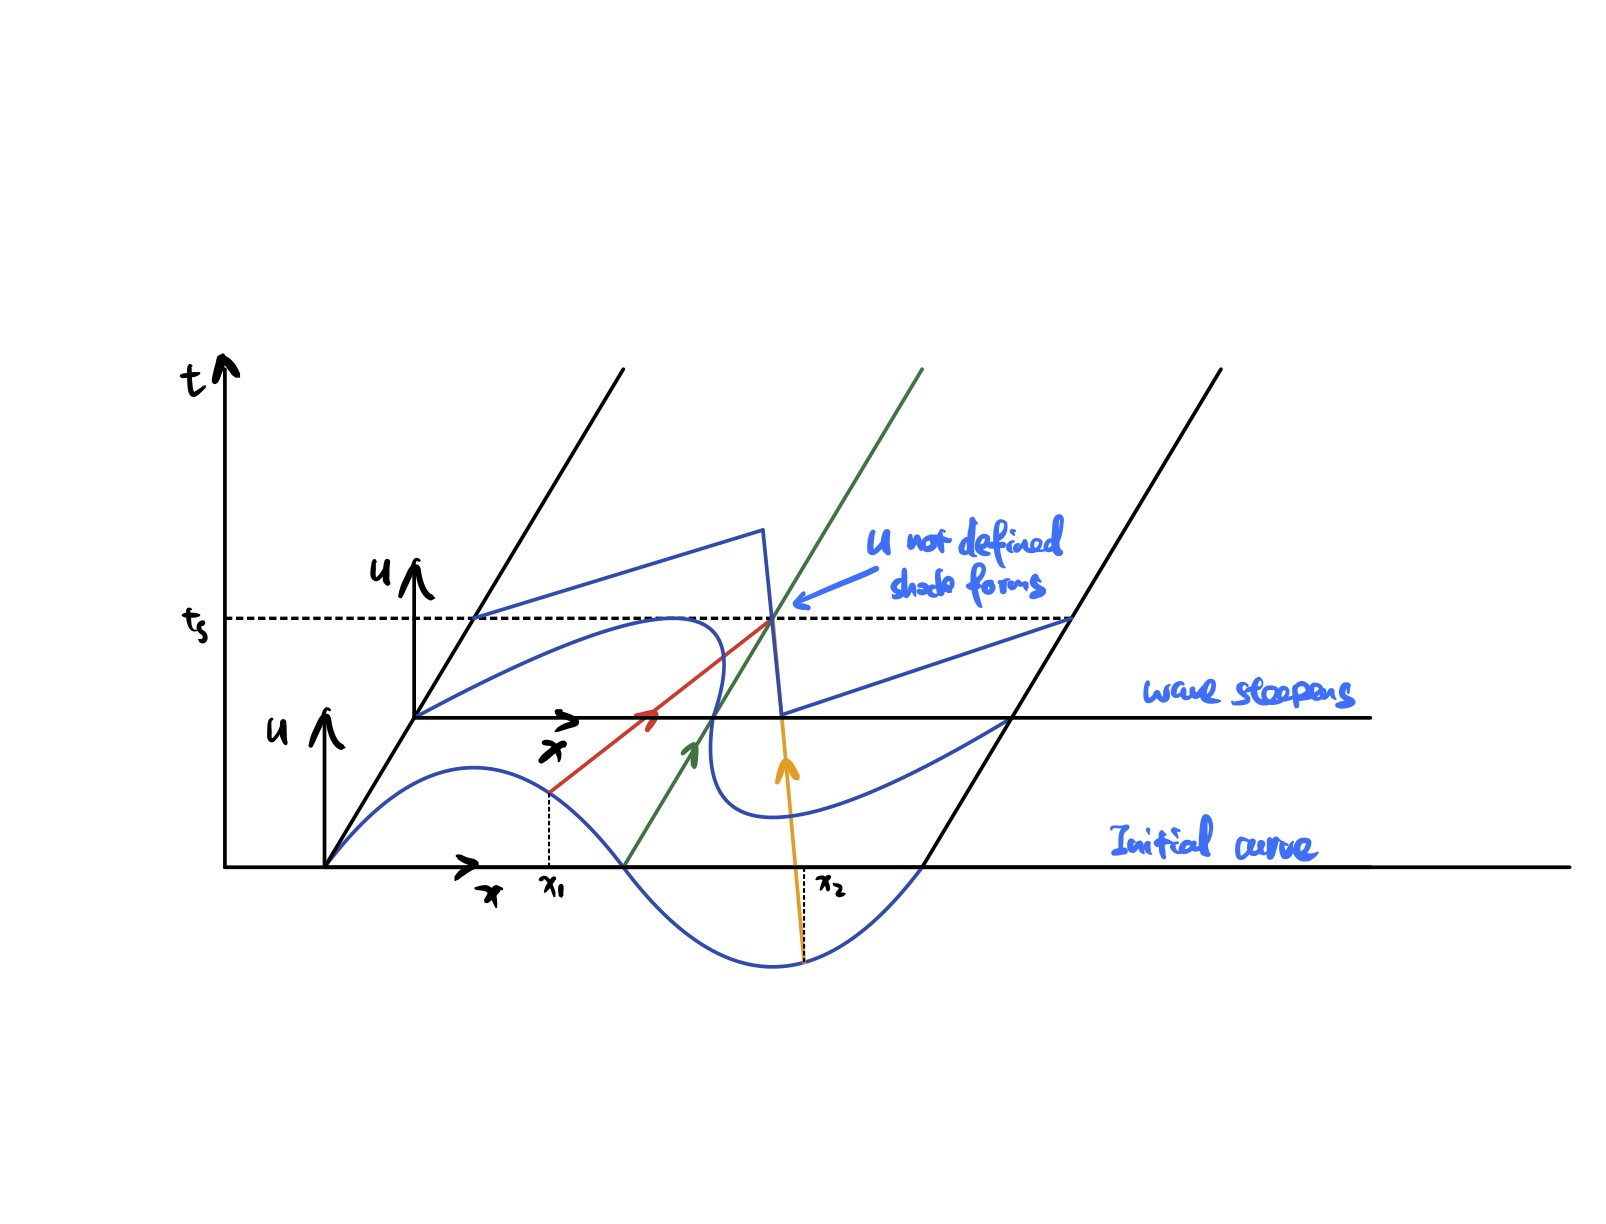
\includegraphics[width = 0.9\linewidth, height =8cm]{Q1.jpg}
 \caption{Figure 1.1: Shock formation with initial data $sin(x)$}
 \label{Q1(1)}
\end{figure}
Since the characteristics (yellow and red) cross,  at $t_s$ , the position x becomes indistinguishable from the initial position $x_0$, and we have $\frac{\partial x}{\partial t} \to 0$ as $t \to t_s$. From \ref{Q1(1)} and also by chain rule we can conclude $\frac{\partial u}{\partial x} = \frac{\frac{du}{dx_0}}{\frac{\partial x}{\partial x_0}} \to \infty$. The condition for a shock to form is that there exists $t_s$ such that $\left. \frac{\partial x}{\partial t}  \right|_{t_s} = 0$. Assume at $t = t_s$ a shock is formed for the first time, then by the characteristic equation, $t_s = \frac{1}{max_{x_0}\left(-\frac{du}{dx_0}(x_0,0)\right)}$.\\
Suppose we have $u(x,0) = const.$, then there is clearly no shock formation as all characteristics are parallel. Suppose we have $u(x,0) = H(x)\ln(x+1)$, then there is no shock either, as t is positive and the characteristics have decreasing gradients as x grows. They don't intersect. 
\newpage
\begin{figure}[H]
 \center
 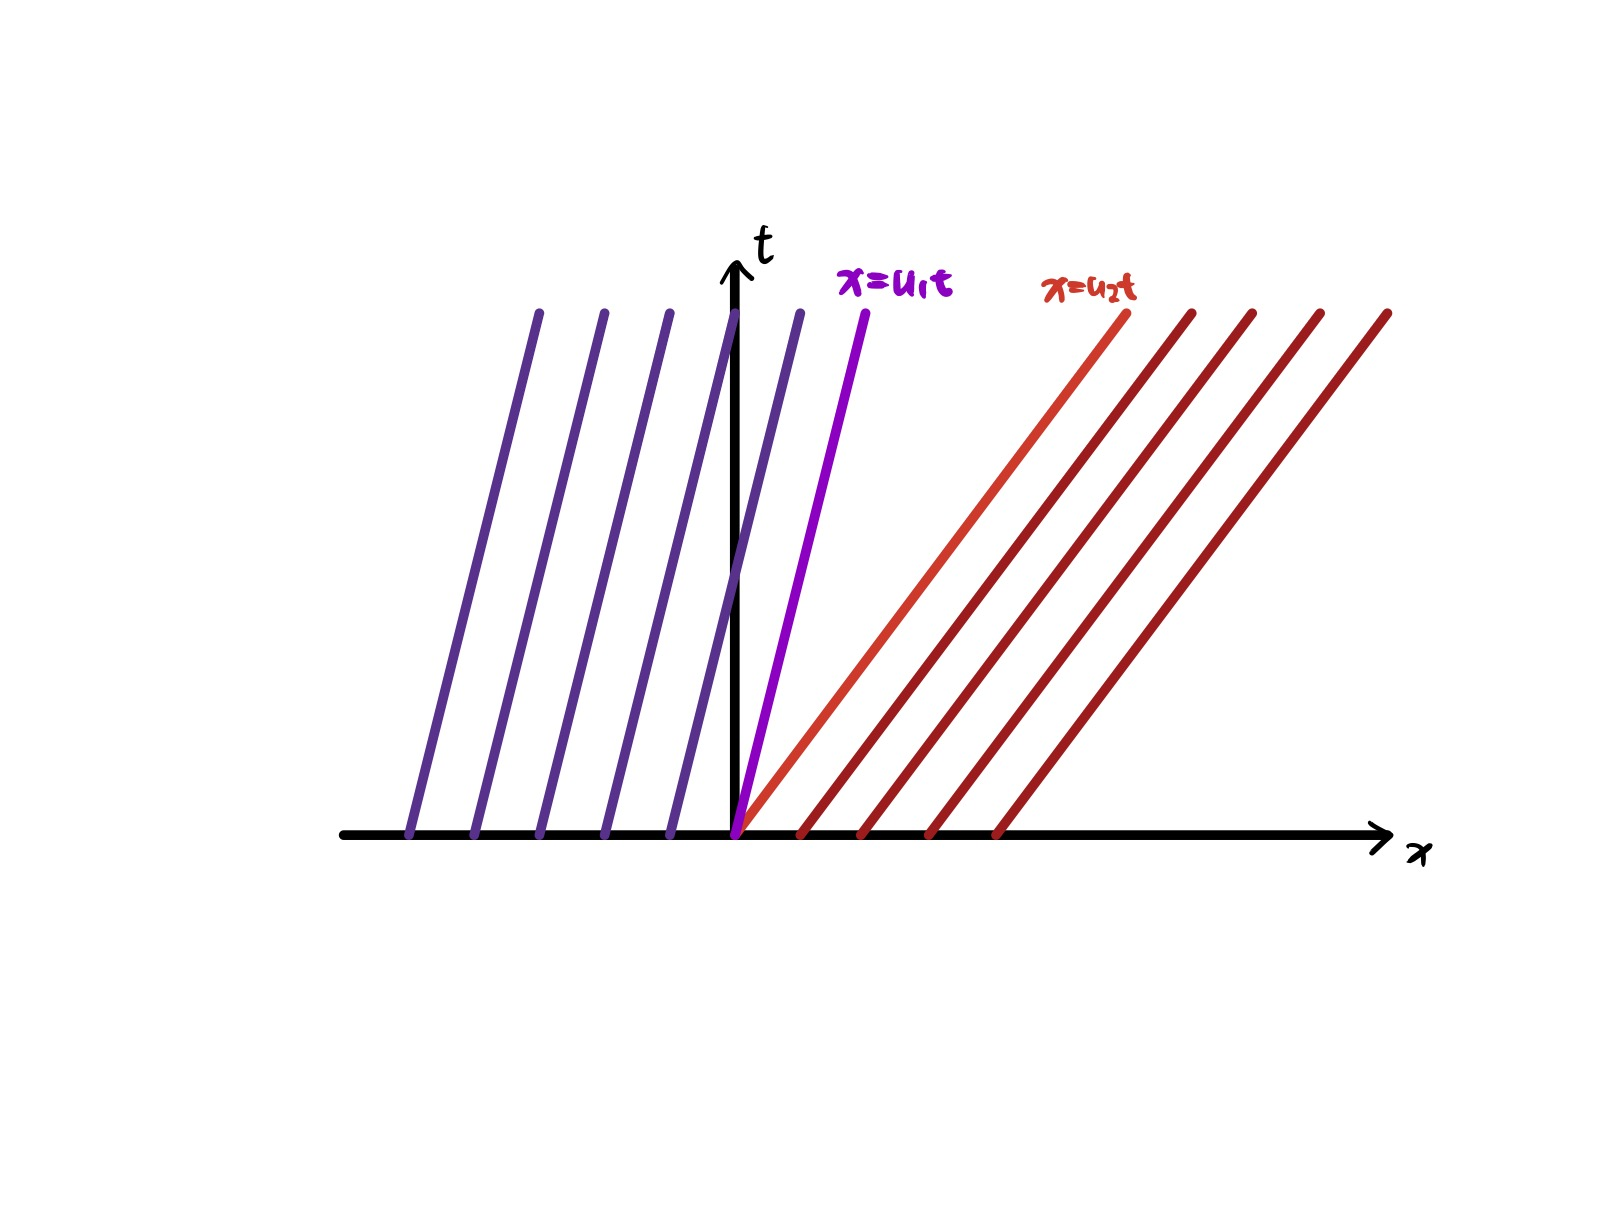
\includegraphics[width = 0.9\linewidth, height =8cm]{Q1(2).jpg}
 \caption{Figure 1.2: Characteristics of step-like Initial data}
 \label{Q1(2)}
\end{figure}
Given the initial condition:
\[
 u(x,0)=\begin{cases}
               u_1 & x < 0\\
               u_2 & x > 0\\
            \end{cases}
\]
with  $u_1<u_2$.
One weak solution is 
\[
 u(x,t)=\begin{cases}
               u_1 & x<u_1 t\\
               \frac{x}{t} & u_1 t<x<u_2 t\\
               u_2 & x>u_2 t\\
            \end{cases}
\]
The other weak solution is a shock wave, since the characteristics travel away from the shock, it is not casual, hence not possible. 
From figure \ref{Q1(2)} there is no possibility of shock formation as the characteristics do not intersect.
\section{Question 2}
The characteristics with the given boundary conditions can be found in \ref{Q2}.
\begin{figure}[H]
\center
 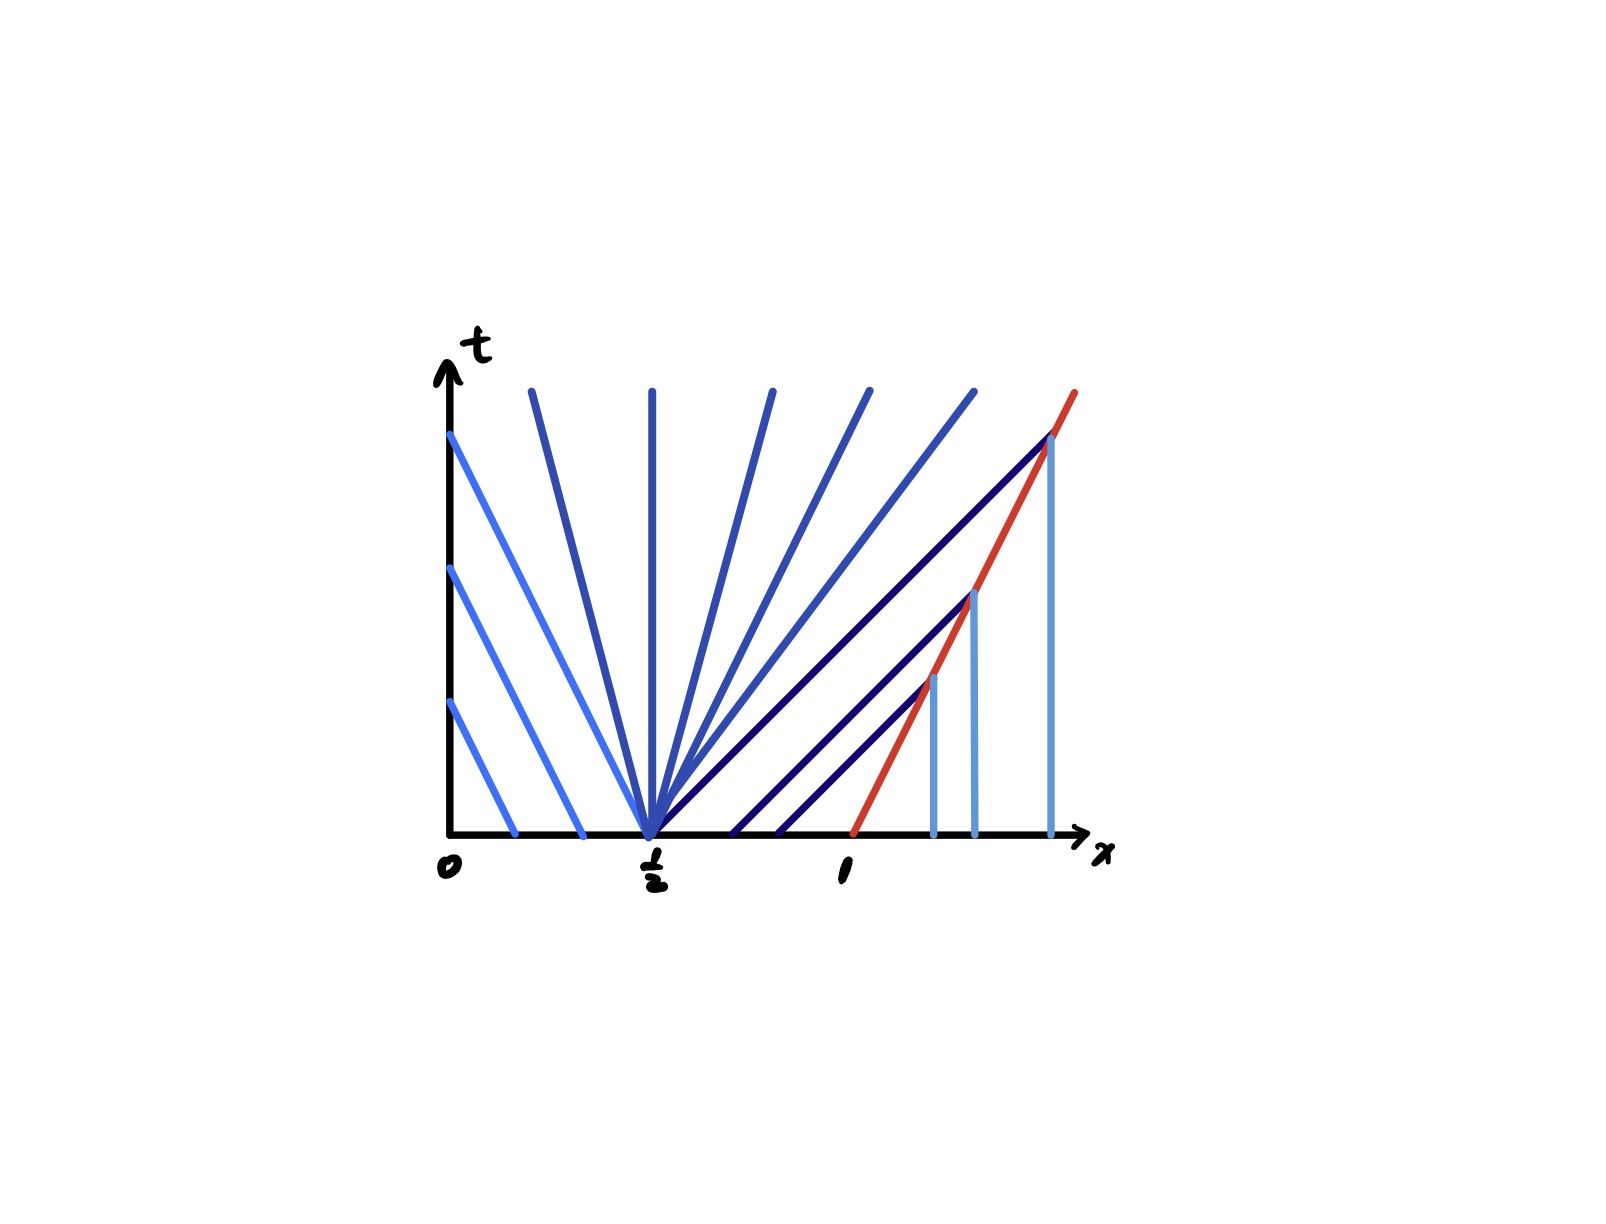
\includegraphics[width = 0.9\linewidth, height =8cm]{Q2.jpg}
\caption{Figure 2.1: characteristics of the initial data (2)}
\label{Q2}
\end{figure}
\begin{figure}[H]
 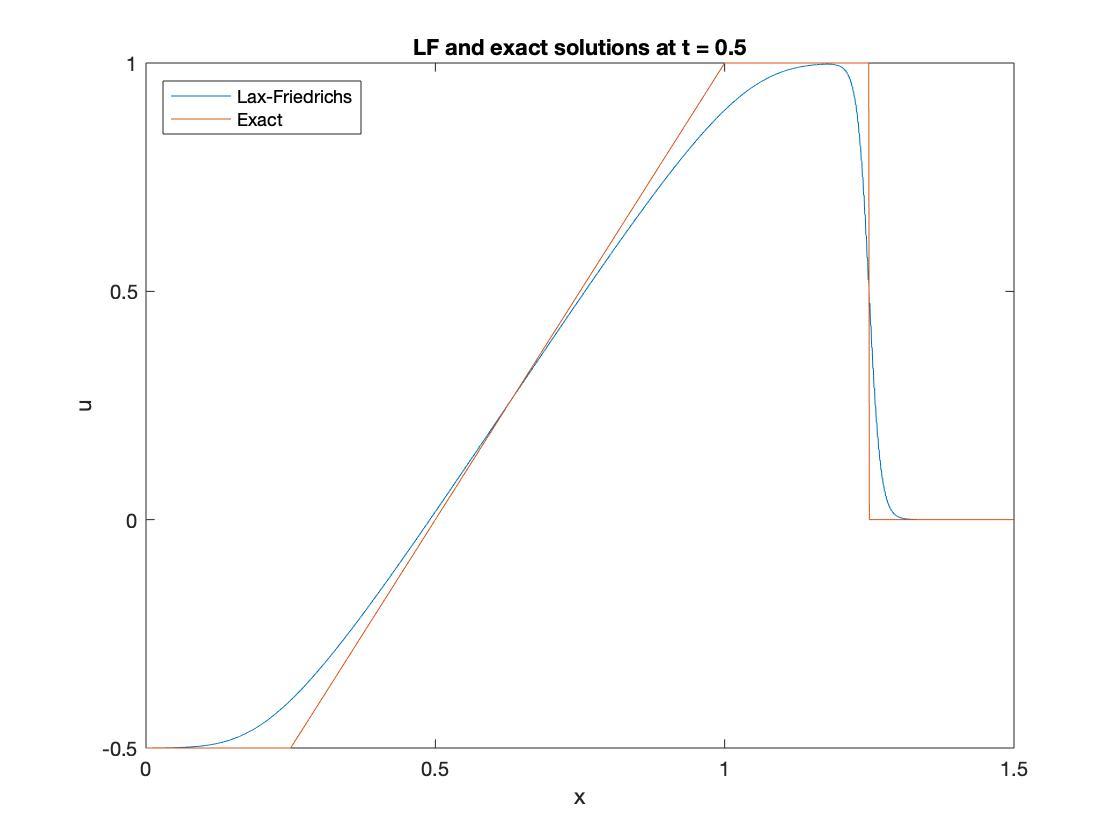
\includegraphics[width = 0.9\linewidth, height =8cm]{Q2(1).jpg}
\caption{Figure 2.2: Exact solution and Lax-Friedrichs scheme at t = 0.5}
\label{Q2(1)}
\end{figure}
\newpage
At $x_0 = 1$ there is a shock. By Rankine-Hugoniot: $$\frac{dx}{dt} = \frac{\left[u^2\right]_{-}^{+}}{2\left[u\right]_{-}^{+}} = \frac{u^{+} +u^{-}}{2} = \frac{1}{2},\;x_0 = 1 $$ 
Therefore the solution is: when $t\leqslant 1$
\[
 u(x,t)=\begin{cases}
               -\frac{1}{2} & x< \frac{1-t}{2}\\
               \frac{2x-1}{2t} & \frac{1-t}{2}\leqslant x<t+\frac{1}{2}\\ 
               1 & t+\frac{1}{2}\leqslant x <\frac{t}{2}+1 \\
               0 & x\geqslant \frac{t}{2}+1\\
            \end{cases}
\] 
and when $t>1$
\[
 u(x,t)=\begin{cases}
               -\frac{1}{2} & x< \frac{1-t}{2}\\
               \frac{2x-1}{2t} & \frac{1-t}{2}\leqslant x<\frac{t}{2}+1\\ 
               0 & x\geqslant \frac{t}{2}+1\\
            \end{cases}
\]
The numerical solution is as in \ref{Q2(1)}. By calculating the truncation error analysis. By \cite{Toro}, the order of accuracy of the scheme is defined as the error caused by approximating the time derivative. We have $$kT_{h}^{k} = k(u_t +(f(u))_x) + k^2 u_t - \frac{h^2}{2} u_{xx} + \mathcal{O}(kh^2), $$ $$ i.e.\ T_{h}^{k}= k u_t - \frac{h^2}{2k} u_{xx} + \mathcal{O}(h^2+k^2).$$ Therefore, the order of accuracy is $\mathcal{O}(k+\frac{h^2}{k})$ and hence Lax-Friedrichs scheme is of first order. It can be shown similarly that the Richtmyer scheme is of second order.
\section{Question 3}
\begin{figure}[H]
 \center
 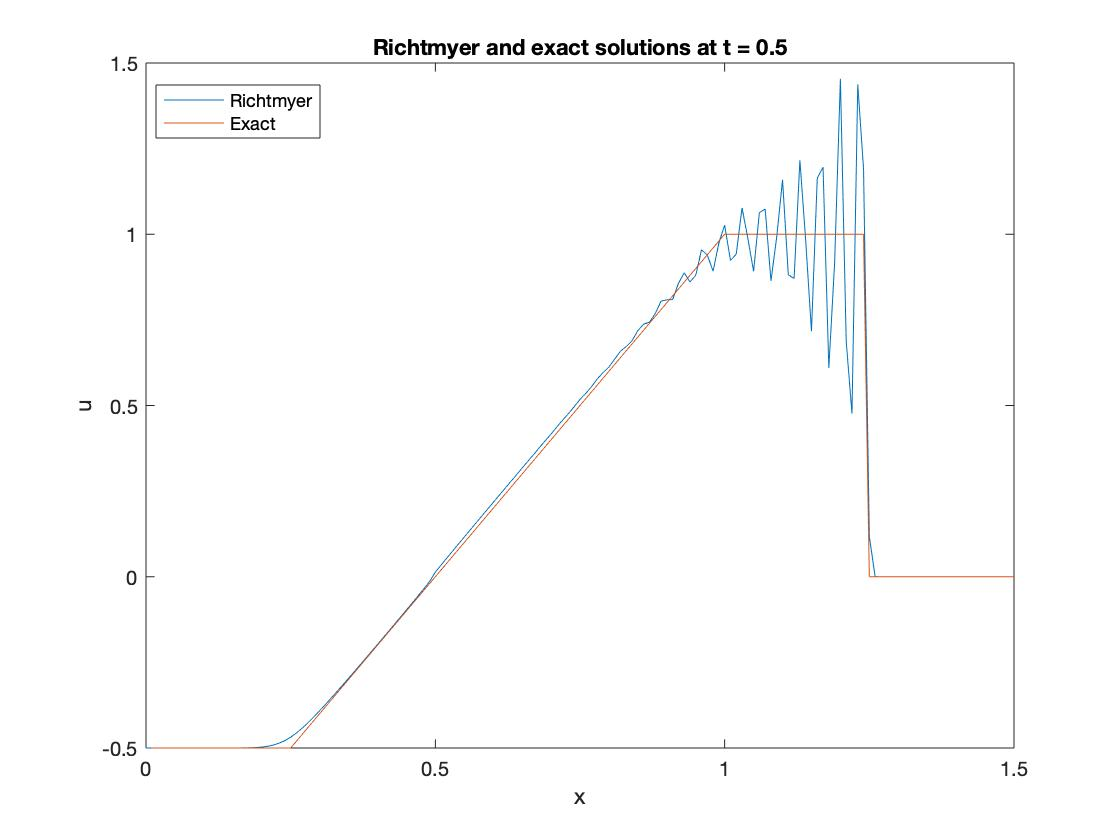
\includegraphics[width = 0.9\linewidth, height =8cm]{Q3.jpg}
 \caption{Figure 3.1: Exact solution and Richtmyer scheme at t = 0.5}
 \label{Q3}
\end{figure}
From Figure 3.1 it is clear that there are spurious oscillations near the point of discontinuity, which causes the inaccuracy of the numerical method near points of high gradient. At the same time, the Richtmyer scheme is more accurate at places where the solution is smoother, as a result of its higher order of accuracy.\\
From p.437 of \cite{Toro}, a scheme $$u_{i}^{n+1} = H(u^{n}_{i-k_L +1}, \cdots, u^{n}_{i+k_R})$$ with $k_L$ and $k_R$ non-negative integers is said to be monotone if $$ \frac{\partial H}{\partial u_j^n} \geq 0\; \forall j$$. For conservation laws, this is just a discrete version of the property that the order of two different initial data is preserved, which is the case for the exact solution. Also from \cite{Toro}, on p.439, it is shown that the Lax-Friedrichs method is monotone, and it can also be shown that Richtmyer is not monotone \footnote{One can argue that because of the Godunov's Theorem (p.444), and the fact that the Richtmyer scheme is second order, it is not monotone.}, which is the cause of the spurious oscillations near the discontinuity.
\section{Question 4}
For a more careful treatment please refer to 13.7 of \cite{Toro}
\begin{enumerate}[label = (\roman*)]
\item
If there is sharp change in the gradient at a point x, we choose a \textbf{small} neighbourhood of it. If the sign is preserved, for some i such that $ih\leqslant x< (i+1)h$, we have $|u^n_{i+1}-u^n_i |\gg|u^n_i -u^n_{i-1}|$ and  $|u^n_{i+1}-u^n_i |\gg|u^n_{i+2} -u^n_{i+1}|$. Then we have $r_i^n \approx 0$, and thus $F \approx F^{LO}$. If the sign is reversed, then$r_i^n = 0$, and $F = F^{LO}$. Therefore, the overall flux is predominantly low order accurate.
\item
If there is slight change in gradient at a point x, then in a \textbf{small} neighbourhood \footnote{small in the sense that any swap of sign is excluded} of it, for some i such that $ih\leqslant x< (i+1)h$, we have $|u^n_{i+1}-u^n_i |\approx|u^n_i -u^n_{i-1}|$ and $|u^n_{i+1}-u^n_i |\approx |u^n_{i+2} -u^n_{i+1}|$. Then we have $r_i^n \approx 1$, and thus the overall flux $F \approx F^{HI}$, which is predominantly high order accurate.
\end{enumerate}
It is desirable because we can choose the low order flux to be a monotone one, and the high order flux to be one with order of accuracy $\geqslant 2$. Therefore, in places where there are sharp changes in gradient, we have a monotone method and hence no spurious oscillations; in places where there are slight changes in gradient, we have a high order method hence higher resolution. 
\section{Question 5}
\begin{figure}[H]
 \center
 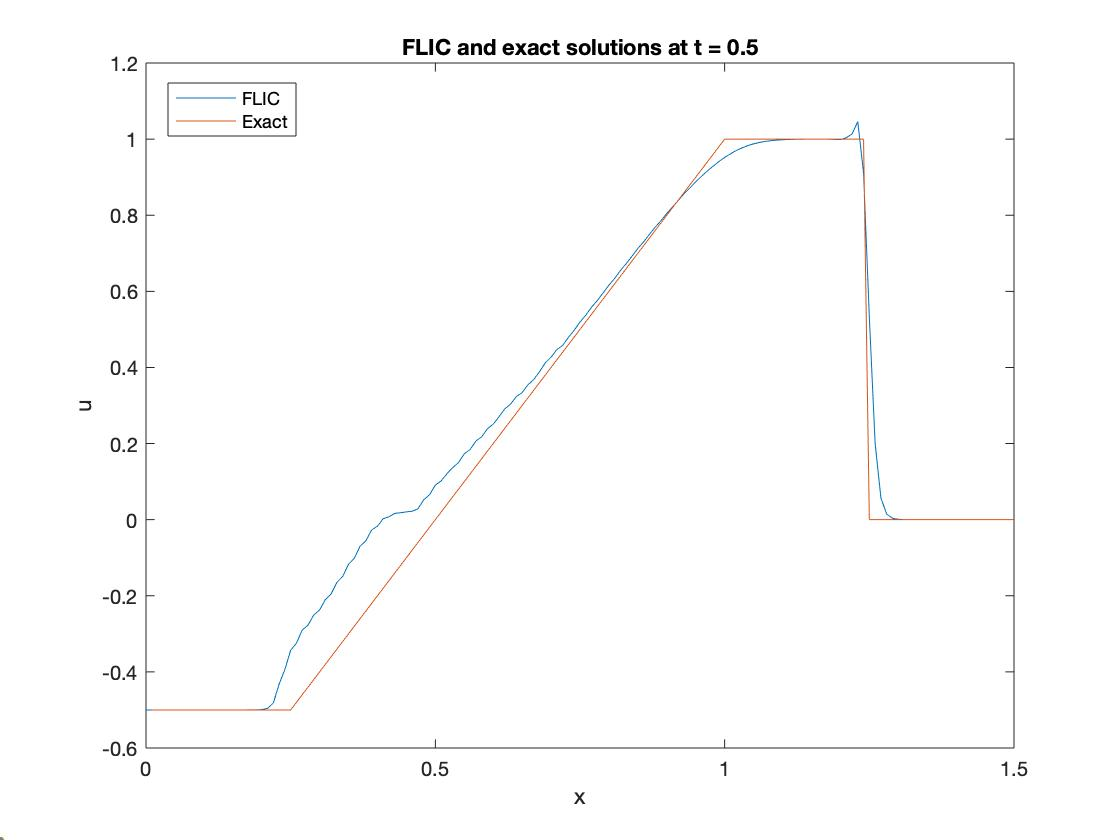
\includegraphics[width = 0.9\linewidth, height =8cm]{Q5.jpg}
 \caption{Figure 5.1: Exact solution and FLIC scheme at t = 0.5}
 \label{Q5}
\end{figure}
By comparing with \ref{Q1(2)} and \ref{Q2(1)}, though it does not fit better than the previous schemes at all points, the scheme has worked better at the discontinuity. Clearly the error is smaller there and there has been no spurious oscillations. For a better scheme we may try other limiter functions.


\begin{thebibliography}{9}
\bibitem{Toro} 
Toro, E.F.
\textit{Riemann Solvers and Numerical Methods for Fluid Dynamics: a practical introduction} 
Springer-Verlag, 1999.
\end{thebibliography}
\newpage
\appendix
\section{Codes}
\subsection{P1}
\label{P1}
\lstinputlisting{Q2.m}
\subsection{P2}
\label{P2}
\lstinputlisting{Q3.m}
\subsection{P3}
\label{P3}
\lstinputlisting{Q5.m}

\end{document}